\section{Component Type Hierarchy}
\label{sec:ComponentTypes}

--------------------------
TODO:
Der Abschnitt muss wieder an die richtigen Stellen in diesem Abschnitt:
Required interfaces of the provided-type are not considered explicitly. However,
if they are specified, their meaning corresponds to the first case in the list,
since, for provided-types, the use of external services is not limited. The
second case corresponds to the complete-type. The usage of external services is
limited to the required interfaces specified for the component and no further
interfaces can be used by the component. The last case expresses additional
component requirements. For example, we could specify that all information has
to be stored in a database. So, the interface of the database must be called
using certain call sequences.
--------------------------

The different meanings of provided and required interfaces and the possiblity
to specify the inner structure of a software component using UML 2.0 and/or
Parametric contracts brings up the question of substitutability. What has to be
fulfilled by a software component that shall replace another component in its
context?

To answer this question is not an easy task, especially, if we want to allow
different meanings of required and provided interfaces and support the analysis
of QoS attributes. We need a component type system that supports different
kinds of substitutability and, furthermore, handels QoS relevant information.

Current component meta models address this issue only
briefly. Furthermore, most of them do not clearly distinguish between components
and component types. For example, the UML 2.0 states:

\begin{quote}
``$[\ldots]$ a component serves as a type whose conformance is defined by these
provided and required interfaces $[\ldots]$. One component may therefore be
substituted by another only if the two are type conformant
\cite[p.142]{OMGUML2005a}.''
\end{quote}

Here, the terms \emph{component type} and \emph{conformance of components and
types} are introduced, but their meaning is not further clearified. Within the
scope of the UML 2.0 superstructure components and component-types are actually
treated equivalently \cite{stand-irgendwo-in:OMGUML2005a}. This might be
approapriate in many cases, but might lead to a blury concept of software
components.

In the following, we introduce the component type hierarchy as it is used by the
Palladio Component Meta Model. There, we distingish the
provided-component-type and complete-component-type as two different type
concepts for software components. Additionally, we consider a
component-implementation-description that specifies the internal structure of a
component.

\begin{figure}[htbp]
\centering
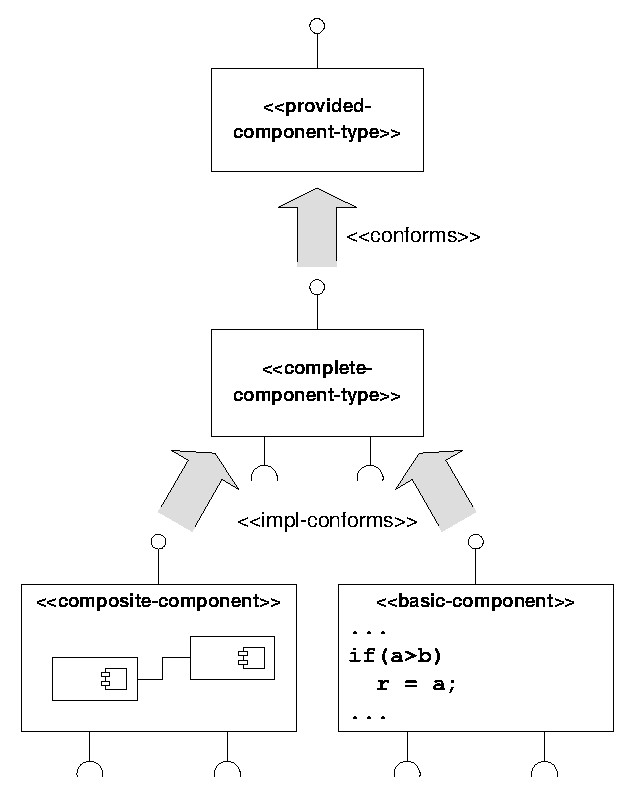
\includegraphics[width=3.3in]{example/Overview_TypeHierarchie}
\caption{Different type levels of a software component.}
\label{fig:TypeOverview}
\end{figure}

Figure \ref{fig:TypeOverview} shows the component type
hierarchy. The provided-component-type is mainly characterised by provided
interfaces. In addition, the complete-component-type considers
required interfaces that can be used by an implementation of the type. We allow
different kinds of component implementation descriptions: Basic components
and composite components. Basic components describe the intra-component
dependencies of provided and required interfaces using parametric contracts.
Composite components are used to construct new components out of other
components.

There are mainly two different concepts of component types. Both differ in
their interpretation of substitutability. 

The first one originates from object
oriented software development. There, a class can be substituted by another if
it implements the same interfaces. Translating this view to the
world of software components, a component can be substituted by another if it
offers at least the same set of provided interfaces.

The second one does not only consider provided interfaces, but also the
required interfaces of a component.

Depending on the task, both concepts have their advantages and disadvantages.
Thus, we do not want to limit on one of the concepts.

Both concepts specify the required interfaces of a software component. However,
the interpretation of a required interface is completely different.



The Palladio Component Meta Model combines the two concepts of component types
and the different meanings of required interfaces to provide a more flexible
type system for components.



During design time, it is often not clear what other components will be needed
to implement the desired functionality. Expecting the software architect to
decide this would require nearly the same effort as implementing the software
component. Thus, the development process of a component should not be fixed to
the required interfaces specified by a complete-component-type. It rather
evolves with the development of the component. Provided and required interfaces
are added and removed over time. The system architect specifies a basic set of
interfaces that is used by the components to communicate. More interfaces might
be added later to implement the functionality of the components.

The distinction of provided- and complete-types brings several advantages. By
provided-types, we gain a high flexibility during software development.
Furthermore, we can define a substitutability focussing on the functionality of
a component. On the other hand, complete-types define a strict substitutability.
If a component is replaced by another and both conform to the same complete
type, we can assure that certain classes of interoperability problems cannot
occur. Moreover, complete-types allow a complete specification of the externally
visible behaviour of a software component. The co-existence of both concepts
offers a high flexibility in software architecture design.


\subsection*{Web Server}
In the following, we describe the concepts mentioned above in more detail. To do
so, we use the architecture of a prototypical web server shown in figure
\ref{fig:WebserverComponents}. The web server has been implemented in C\#
using the Microsoft .Net 1.1 framework. It consists of a set of components that
communicate via a clear defined set of interfaces only. The web server uses all
concepts relevant for component based software development. Moreover, its
architecture is comparable to many three tier applications.

\begin{figure}[htbp]
\centering
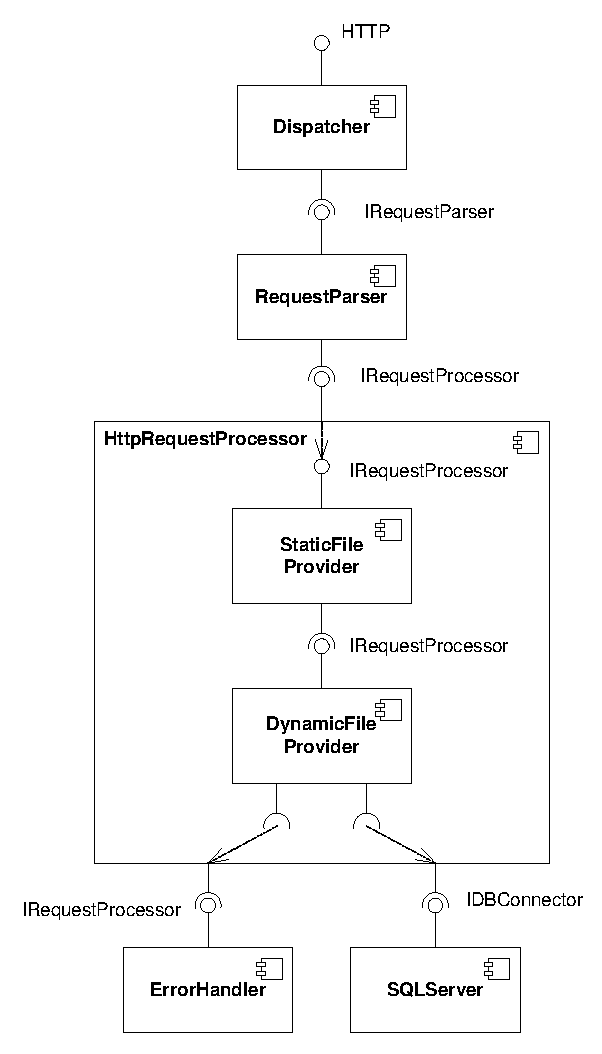
\includegraphics[width=3.3in]{example/WebserverComponents}
\caption{Component architecture of a web server.}
\label{fig:WebserverComponents}
\end{figure}

The main part of the web server is realised by three components: Dispatcher,
RequestParser, and HttpRequestProcessor. The Dispatcher listens for
incoming connections. For each HTTP request, it spawns a new thread and
activates the RequestParser. The parser analyses the request and passes the
result to the HttpRequestProcessor. The request processor is organised as a
Chain of Responsability \cite{gamma1995a}. Each of its subcomponents checks
whether it can handle the incoming request. If so, it returns the result,
otherwise it passes the request to the next component in the chain of
responsibility. The ErrorHandler component represents the end of the chain and
returns an error message if the request could not be handled by any of the
components. Additionally, the SQLServer is required to create dynamic HTML
pages.

\subsection*{Component Implementation Description}
Today's understanding of software components is strongly influenced by
state-of-the-art technologies, like J2EE, CORBA, and COM+.
Most software architects think of a software component as a 'physical thing',
like a piece of code, a special kind of class, or a binary file. All of them
realise a certain functionality and have special requirements to the
environment in order to function correctly.
The component implementation description specifies the provided and required
interfaces and the inner structure of such components.

A component implementation description is always associated with at least
one binary ('physical') component. Certainly, multiple implementations
can exist for a single description. For example, the same
specification can be implemented in different programming languages like Java
and C\# and/or component technologies, like CORBA, J2EE, or COM+. 

Different possibilities exist to specify the internal structure of a
component. For example, the UML 2.0 superstructure \cite{OMGUML2005a} allows to
describe the inner component structure as a class diagram.
On the other hand, parametric contracts specify the dependency of provided
and required interfaces by means of service effect specifications.
Moreover, some components are constructed by composing other components. These
inner components and their interconnection are also a representation of the
inner component structure.

In this article, we focus on the component implementation description with
parametric contracts and composite structures, since our main aim is the
prediction of QoS attributes. Both concepts have been proofed to be beneficial
for this task. Thus, we distinguish between two types of component
implementation descriptions: Basic components and composite components.

A \emph{basic component} represents a basic block that is not further
subdivided. It implements a certain functionality and is defined by its provided
interfaces, required interfaces, and service effect specifications.

The fact that a basic component represents a single block does not imply that
the real implementation has to be one 'block' as well. Since we are talking
about the implementation description and not the actual implementation, this
difference is possible and actually desired in some cases. For example, the
actual implementation of a component might consist of a set of classes. This
information is abstracted away in the description as a basic component. In
the web server example shown in figure \ref{fig:WebserverComponents}, the
components StaticFileProvider and DynamicFileProvider are described as basic
components.

\begin{figure}[htbp]
\centering
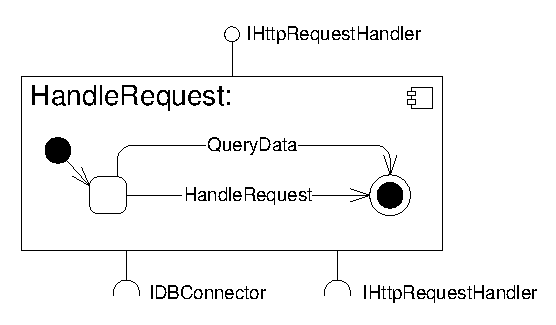
\includegraphics[scale=0.85]{example/HandleRequestSEFF}
\caption{Service effect specification of the method HandleRequest in the
DynamicFileProvider.}
\label{fig:seff}
\end{figure}

Figure \ref{fig:seff} shows the service effect specification of the method
HandleRequest of the DynamicFileProvider modelled as a
finite state machine. If the DynamicFileProvider is responsible for the incoming
request, it executes a query on the connected database. It uses the queried
information to construct the web page and returns the result to the client.
This is realised by internal component code that is not modelled by the
service effect specification shown in figure \ref{fig:seff}. If the
DynamicFileProvider is not responsible for the incoming
request, it forwards it to the next component in the chain of
responsibility. This is done by the call of the HandleRequest method of the
component connected to the IHttpRequestHandler interface.

A component cannot only be implemented by writing source code that realises the
desired functionality, but also by composing components. We explicitly consider
the composition of components and the writing of source code as equivalent
means of implementation.

A \emph{composite component} consists of a set of interconnected subcomponents
that realise its functionality \cite[TODO:page]{OMGUML2005a}. 

As in UML 2.0, the interconnection of the inner components is realised by
assembly connectors while delegation connectors describe how the externally
visible interfaces are mapped to the inner structure of the component.

It is important to mention that the composite structure of a component can be
hidden from the deployer. The service effect specifications of a composite
component can be computed out of the inner components and their interconnections
\cite{TODO:Reference FESCA paper}. Unfortunately, composite components can
hardly be represented with today's component technologies. The construction of a
new component out of existing components can often only be done manually. So,
composite components remain logical constructs in most cases. More sophisticated
technologies are needed, which offer an easy way to hide the inner structure of
composite components and generate its physical representation.

The HttpRequestProcessor is the only composite component shown in the
architecture of the web server in figure \ref{fig:WebserverComponents}. It
contains a set of different request processors that are organised in
a  Chain of Responsability. This hides the different processors from the other
components and presents them as a single entity to the outside world.

Next, we introduce the complete component type as a more abstract view on
software components.


\subsection*{Complete Component Type}

A complete component type generalises the component implementation description
by omitting the inner structure of a component. Thus, it only contains provided
and required interfaces.

\begin{figure}[htbp]
\centering
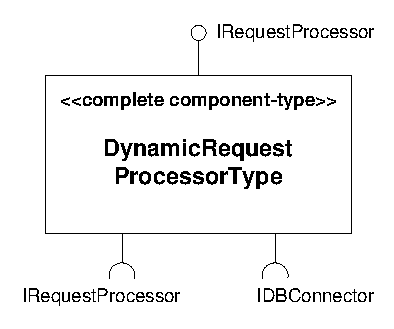
\includegraphics[scale=0.85]{example/DynamicRequestProcessorType}
\caption{Component complete type for dynamic request processors.}
\label{fig:DynamicRequestProcessorType}
\end{figure}

Looking at the architecture of the web server, we can identify different
complete component types. For example, the components HttpRequestProcessor and
DynamicFileProvider provide the IRequestProcessor interface and use the
interfaces IDBConnector and IRequestProcessor. The first one is used to retrieve
dynamic content of web pages from a data base. The second one is required to
forward the request to the next component in the chain of responsibility. The
corresponding type of
both components is shown in figure \ref{fig:DynamicRequestProcessorType}.

\begin{figure}[htbp]
\centering
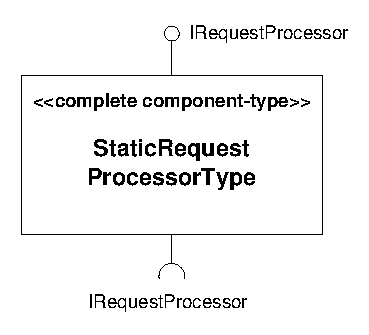
\includegraphics[scale=0.85]{example/RequestProcessorType}
\caption{Another component type used in the web server.}
\label{fig:RequestProcessorType}
\end{figure}

The type of the StaticFileProvider component shown in figure
\ref{fig:RequestProcessorType} provides and requires the IRequestProcessor
interface only. So, it differs from the DynamicRequestProcessorType, which
additionally requires the IDBConnector interface. 

The types shown in figures \ref{fig:DynamicRequestProcessorType} and
\ref{fig:RequestProcessorType} are derived from existing components and describe
their complete provided and required functionality. A component conforms to a
type if it provides and requires exactly the interfaces specified by the type.
This very basic definition of conformance is not sufficient for a type system
of component. A component is likely to differ from its more general type, but,
nevertheless, still be conformant to the type. Thus, we can define the
conformance relation between a component implementation description and a
complete component type as follows:

A component implementation description conforms to a complete component type, if
it offers at least the functionality specified by the provided interfaces of the
type and uses only the functionality specified by the required interfaces of the
type. This type of conformance is labelled with the UML stereo-type
$\ll$implementation-conforms$\gg$.

For example, a component must offer the IRequestProcessor interface to conform
to one of the types in figure \ref{fig:DynamicRequestProcessorType} or
\ref{fig:RequestProcessorType}, but it can provide additional interfaces.
Furthermore, a component can only use services that are specified in the
required interfaces of the type. The DynamicFileProvider does not conform to the
RequestProcessorType, since it uses the IDBConnector interface. Note that a
component does not have to use all required interfaces of its type. So, all
components that conform to the RequestProcessorType also conform to the
DynamicRequestProcessorType, since they do not require the
IDBConnectorInterface. 

The definition of conformance corresponds to the view on required and provided
interfaces as pre- and postconditions of components. The precondition can only
be weakened. Thus, the component implementation must not use interfaces other
than the required interfaces specified by the type. Furthermore, the
postcondition can only be strengthened. The component can offer any interfaces,
but it must at least provide the ones specified by the type. With this notion of
conformance, the type system of components is contravariant.

The relation $\ll$implementation-conforms$\gg$ allows us to
define substitutability of components. A component \texttt{A} can be substituted
by a component \texttt{B} if the description of \texttt{B} conforms to the type
defined by \texttt{A}. The component complete type defined by a component
and its description includes all its provided and required interfaces.
Therefore, a component implementation description always conforms to at least
the type it defines. This definition of substitutability is very conservative.
It ensures that the new component can function in the existing environment,
but, on the other hand, might be to restictive. Therefore, we introduce the
provided component type next, which allows a more flexible notition of
substitutability and type conformance.

\subsection*{Provided Component Type}

In many cases, we are not solely interested in the substitution of complete
components including provided and required interfaces, but in a substitution
with respect to provided interfaces only. This is the case if the functionality
is more important than the requirements of a component or if we compare the
functionality offered by different components. This view is strongly influenced
by object oriented programming, where required interfaces and/or classes are
often not listed explicitly. There, substitutability of classes and interfaces
is
defined on the basis of the $\ll$realize$\gg$ and $\ll$extends$\gg$ relations
\cite{TODO: sinnvolle referenz einf�gen}.

\begin{figure}[htbp]
\centering
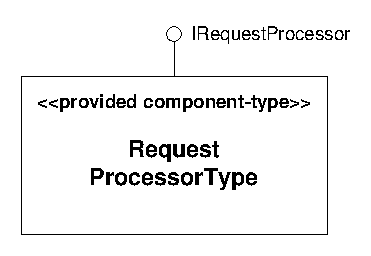
\includegraphics[scale=0.85]{example/ProvidesType}
\caption{provided-type of the RequestProcessorType and
DynamicRequestProcessorType.}
\label{fig:ProvidesType}
\end{figure}

Therefore, we introduce a \emph{provided-component-type}, which only considers
provided interfaces for conformance checks. The provided-component-type of
the RequestProcessortType and the DynamicRequestProcessorType is shown in figure
\ref{fig:ProvidesType}. It only contains the single provided interface
IRequestprocessor. Required interfaces can be specified for the
provided-component-type as well, but their meaning differs from the ones
specified in the complete-component-type. Here, required interfaces are
used in the sense of can-require-interfaces, whose definition does not enforce
any restrictions. Thus, the conformance relation of provided- and
complete-component-types considers provided interfaces only.

A complete-component-type conforms to a provided-component-type, if
it offers at least the functionality specified by the provided interfaces of the
provided-component-type This type of conformance is labelled with the UML
stereo-type $\ll$provided-conforms$\gg$.

Since it exists an equivalent type for each component implementation
description, the $\ll$provided-conforms$\gg$ relation is indirectly defined
between component-implementation-descriptions and provided-component-types.

The provided-implementation-type completes the hierarchy introduced in the
beginning of this section. Next, we summarise the results of this discussion.

\subsection*{The Component Type Hierarchy}

\begin{figure}[htbp]
\centering
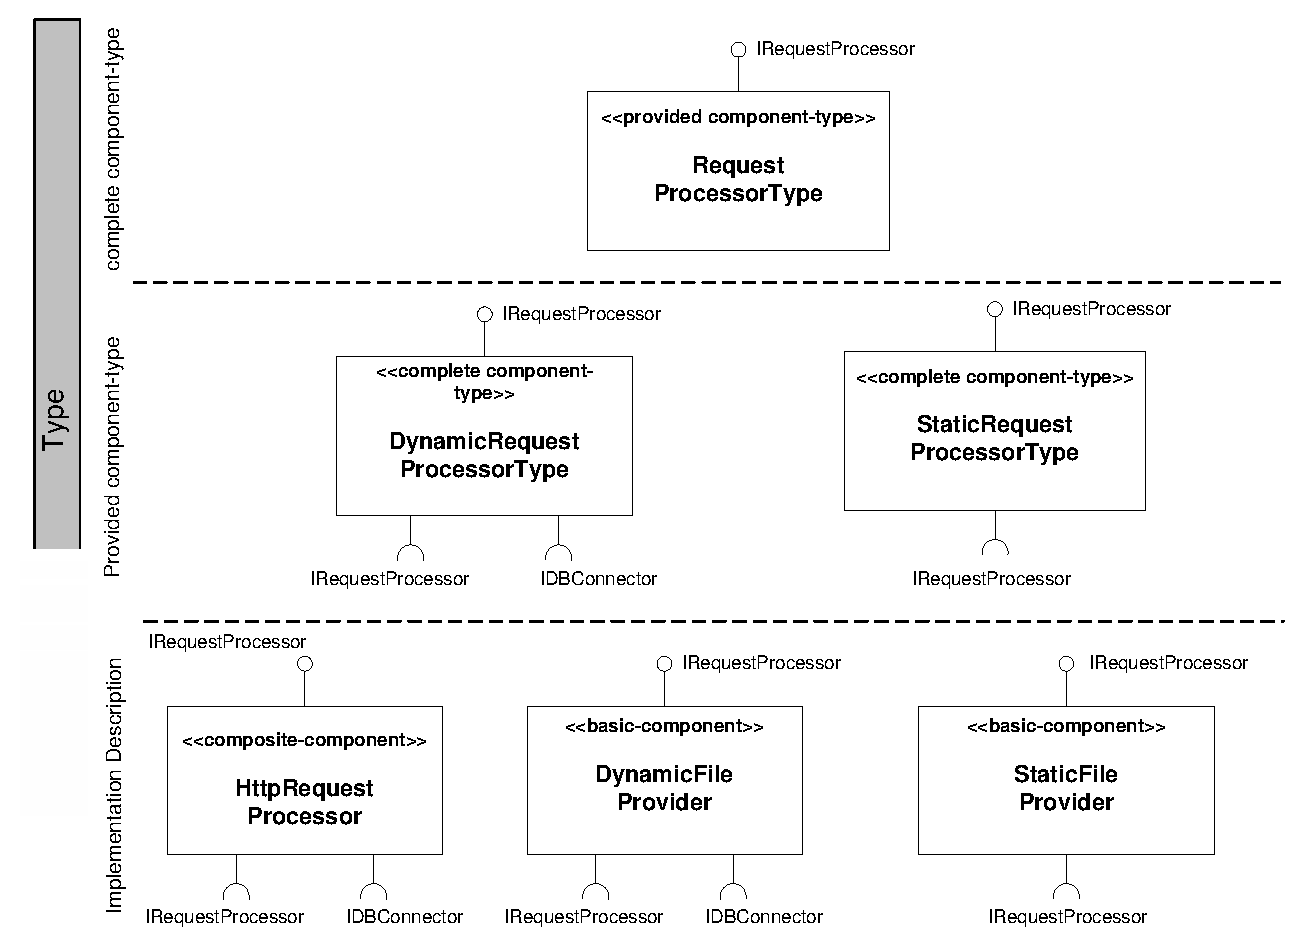
\includegraphics[width=3.3in]{example/TypeHierachy}
\caption{Type Hierarchy}
\label{fig:TypeHierarchy}
\end{figure}

Figure \ref{fig:TypeHierarchy} gives an overview of the relation between
provided-component-types, complete-component-types and component implementation
descriptions. On top of the hierarchy stands the provided-component-type. It is
the most general and flexible view on software components. Its focus is on
provided interfaces. It is also possible to add required interfaces, but
with a very loose semantic. The complete-component-type is placed on
the mid level of the hierarchy. It considers required interfaces
with a more strict semantic, which prohibits the usage of interfaces other
than the specified required interfaces. The component implementation description
on the bottom of the hierarchy adds knowledge about the internal structure of
a component to the model. As indicated by the fading bar on the left hand
side, we do not consider the description as a type. 

With the implementation description of software components, we provide a lot of
information, which allows us to compute QoS attributes with a higher precision.
For example, we can determine the influence of the QoS of required services on
the provided services \cite{TODO: FESCA05, QoSA, reussner2003d}. However, the
QoS attributes are not only influenced by external services, but also by the
underlying hardware and software resources. Thus, our next step is the
modelling of the deployment context.
